\documentclass{article}
\usepackage[dvipsnames]{xcolor}
\usepackage[paperwidth=12cm, paperheight=10cm, margin = 0cm, top=0.5cm]{geometry}
\usepackage{amsmath}


\usepackage{pgf}
\usepackage{tikz}


\usetikzlibrary{arrows,automata, positioning}

\tikzstyle{source}  = [draw,circle,fill=black,thick,inner sep=0mm,minimum size=2mm]

\renewcommand{\vec}[1]{\boldsymbol{#1}}

\begin{document}
\begin{center}
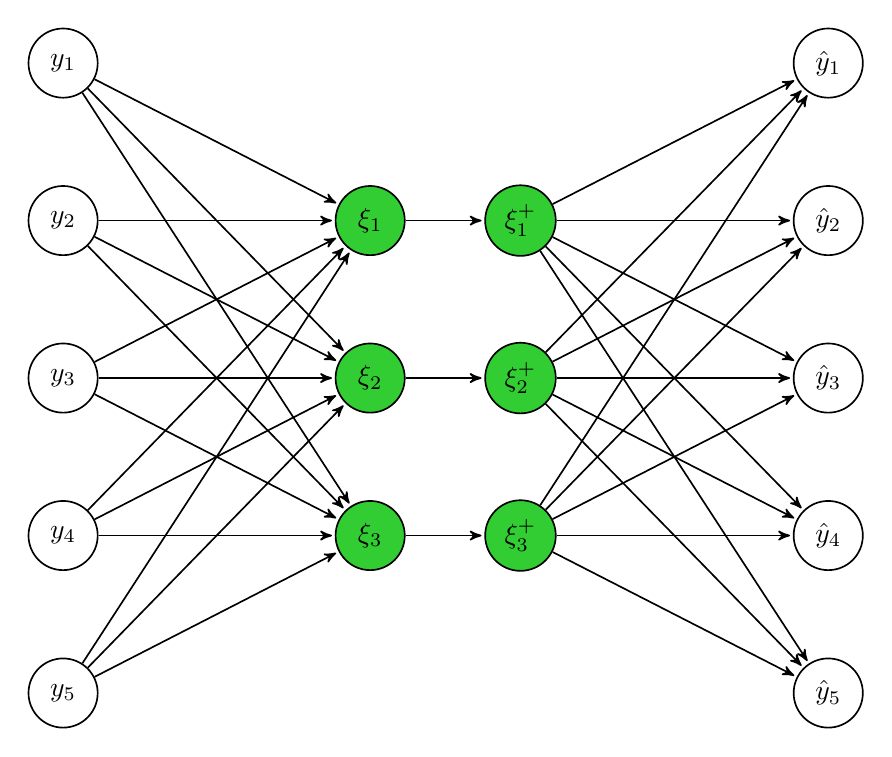
\begin{tikzpicture}[-,>=stealth',shorten >=1pt,auto,node distance=2cm,semithick]
                    
\node[state] (Y1)               {$y_{1}$}; 
\node[state] (Y2) [below of=Y1] {$y_{2}$};                   
\node[state] (Y3) [below of=Y2] {$y_{3}$};                   
\node[state] (Y4) [below of=Y3] {$y_{4}$};                   
\node[state] (Y5) [below of=Y4] {$y_{5}$};                   

\node[state, fill=LimeGreen] (X1) [right=3cm of Y2] {$\xi_{1}$}; 
\node[state, fill=LimeGreen] (X2) [right=3cm of Y3] {$\xi_{2}$}; 
\node[state, fill=LimeGreen] (X3) [right=3cm of Y4] {$\xi_{3}$}; 

\node[state, fill=LimeGreen] (XP1) [right=1cm of X1] {$\xi_{1}^+$}; 
\node[state, fill=LimeGreen] (XP2) [right=1cm of X2] {$\xi_{2}^+$}; 
\node[state, fill=LimeGreen] (XP3) [right=1cm of X3] {$\xi_{3}^+$}; 


\node[state] (Z2) [right=3cm of XP1] {$\hat{y}_{2}$};                   
\node[state] (Z3) [right=3cm of XP2] {$\hat{y}_{3}$};                   
\node[state] (Z4) [right=3cm of XP3] {$\hat{y}_{4}$};                   
\node[state] (Z5) [below of=Z4] {$\hat{y}_{5}$};                   
\node[state] (Z1) [above of=Z2] {$\hat{y}_{1}$}; 

\path (Y1) edge[->] (X1)
      (Y1) edge[->] (X2)
      (Y1) edge[->] (X3)
      (Y2) edge[->] (X1)
      (Y2) edge[->] (X2)
      (Y2) edge[->] (X3)
      (Y3) edge[->] (X1)
      (Y3) edge[->] (X2)
      (Y3) edge[->] (X3)
      (Y4) edge[->] (X1)
      (Y4) edge[->] (X2)
      (Y4) edge[->] (X3)
      (Y5) edge[->] (X1)
      (Y5) edge[->] (X2)
      (Y5) edge[->] (X3);

\path (X1) edge[->] (XP1)
      (X2) edge[->] (XP2)
      (X3) edge[->] (XP3);

\path (XP1) edge[->] (Z1)
      (XP1) edge[->] (Z2)
      (XP1) edge[->] (Z3)
      (XP1) edge[->] (Z4)
      (XP1) edge[->] (Z5)
      (XP2) edge[->] (Z1)
      (XP2) edge[->] (Z2)
      (XP2) edge[->] (Z3)
      (XP2) edge[->] (Z4)
      (XP2) edge[->] (Z5)
      (XP3) edge[->] (Z1)
      (XP3) edge[->] (Z2)
      (XP3) edge[->] (Z3)
      (XP3) edge[->] (Z4)
      (XP3) edge[->] (Z5);

\end{tikzpicture}
\end{center}

\end{document}
